%\documentstyle[epsf,twocolumn]{jarticle}       %LaTeX2e仕様
\documentclass[twocolumn]{jarticle}     %pLaTeX2e仕様(platex.exeの場合)
% \documentclass[onecolumn]{ujarticle}   %pLaTeX2e仕様(uplatex.exeの場合)
%%%%%%%%%%%%%%%%%%%%%%%%%%%%%%%%%%%%%%%%%%%%%%%%%%%%%%%%%%%%%%
%%
%%  基本バージョン
%%
%%%%%%%%%%%%%%%%%%%%%%%%%%%%%%%%%%%%%%%%%%%%%%%%%%%%%%%%%%%%%%%%
\setlength{\topmargin}{-45pt}
%\setlength{\oddsidemargin}{0cm}
\setlength{\oddsidemargin}{-7.5mm}
%\setlength{\evensidemargin}{0cm}
\setlength{\textheight}{24.1cm}
%setlength{\textheight}{25cm}
\setlength{\textwidth}{17.4cm}
%\setlength{\textwidth}{172mm}
\setlength{\columnsep}{11mm}

%\kanjiskip=.07zw plus.5pt minus.5pt


% 【節が変わるごとに (1.1)(1.2) … (2.1)(2.2) と数式番号をつけるとき】
%\makeatletter
%\renewcommand{\theequation}{%
%\thesection.\arabic{equation}} %\@addtoreset{equation}{section}
%\makeatother

%\renewcommand{\arraystretch}{0.95} 行間の設定
%%%%%%%%%%%%%%%%%%%%%%%%%%%%%%%%%%%%%%%%%%%%%%%%%%%%%%%%
%\usepackage{graphicx}   %pLaTeX2e仕様(\documentstyle ->\documentclass)
\usepackage[dvipdfmx]{graphicx}
\usepackage{subcaption}
\usepackage{multirow}
\usepackage{amsmath}
\usepackage{url}
\usepackage{ulem}
\usepackage{algorithm}
\usepackage{algorithmic}
\usepackage{listings} %,jlisting} %日本語のコメントアウトをする場合jlistingが必要
%ここからソースコードの表示に関する設定
\lstset{
  basicstyle={\ttfamily},
  identifierstyle={\small},
  commentstyle={\smallitshape},
  keywordstyle={\small\bfseries},
  ndkeywordstyle={\small},
  stringstyle={\small\ttfamily},
  frame={tb},
  breaklines=true,
  columns=[l]{fullflexible},
  numbers=left,
  xrightmargin=0zw,
  xleftmargin=3zw,
  numberstyle={\scriptsize},
  stepnumber=1,
  numbersep=1zw,
  lineskip=-0.5ex
}
%%%%%%%%%%%%%%%%%%%%%%%%%%%%%%%%%%%%%%%%%%%%%%%%%%%%%%%%
\begin{document}

	%bibtex用の設定
	%\bibliographystyle{ujarticle}

	\twocolumn[
		\noindent
		\hspace{1em}
		2020 年 5 月 8 日
		ゼミ資料
		\hfill
		B4 杉山 竜弥
		\vspace{2mm}

		\hrule
		\begin{center}
			{\Large \bf 進捗報告}
		\end{center}
		\hrule
		\vspace{9mm}
	]

	% ‚ここから 文章 Start!
\section{今週やったこと}
\begin{itemize}
	\item {cnnモデルの改良}
	\item {入れ替えデータの解析}
\end{itemize}

\section{問題設定}
% 何を入力として何を出力とするかを明確に定義

 データを正解と不正解に分割して学習する以下のアルゴリズム1を考える.

	\begin{algorithm}
		\caption{Swap two datasets}
		\label{alg1}
		\begin{enumerate}{ % itemize, enumerate, description
			\item{データ 2N 抜き出す}
			\item{そのデータを N(A) と N(B)に分ける.}
			\item{A → train, B → test で実験}
			\item{B → train, A → test で実験}
			\item{3.と4.で test でミスしたデータを調べる}
			\item{A をテストとしたとき失敗したデータと B をテストとしたとき成功したデータを入れ替える.}
			\item{3.に戻る.}
		}\end{enumerate}
			% \begin{algorithmic}
			% \end{algorithmic}
	\end{algorithm}

	アルゴリズム1の手順6の操作によって, データセットAには成功データ, Bには失敗データが集められる.
	従って簡単なデータを学習し, 難しいデータでテストされる手順3の精度は低くなると予想される.

	アルゴリズム1に示した手順の設定として, 手順 3. 4.で2つのモデルをそれぞれ独立させた. またデータポイントの入れ替えは, 入れ替え可能なデータを先頭から全て交換することにした.


\section{実験}

	\begin{table}[tb]
		\begin{center}
			\caption{実験の設定}
			\begin{tabular}{|c|c|} \hline
				dataset & cifar10 \\
				data N & 25,000 / model \\ \hline
				task & 10クラス識別 \\
				input & image(3x32x32) \\
				output & class(10) \\ \hline
				model & CNN(16層) \\
				optim & SDG (lr=0.001, moment=0.9) \\
				loss & Cross Entropy Loss \\ \hline
				batch size & 16 \\
				epoch & 50 \\ \hline
			\end{tabular}
			\label{tab:setting}
		\end{center}
	\end{table}

予備実験によって, ベースラインを測りパラメータを調整した. 最適化関数をAdamにした場合やバッチサイズを増やした場合などを試したが精度が下がる結果となった.
実験では改良したCNNと学習を50epochまで増やした条件で, 学習を行い, 入れ替えデータを解析した.

\begin{figure}[tb]
	\begin{center}
		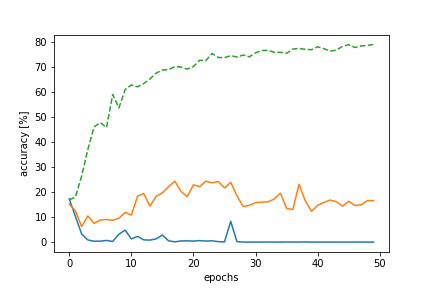
\includegraphics[clip,width=8.5cm]{accuracy.png}
		\caption{テストの精度 (横軸:epoch, 縦軸:精度[\%])
		実線の青が手順3, 橙が手順4,
		点線がベースライン}
		\label{fig:accuracy}
	\end{center}
\end{figure}

図\ref{fig:accuracy}にテストの精度を示した.
ベースラインの学習は期待通り, 80 [\%]の前回より高い精度になった.
一方入れ替えを行った場合, 両方の場合で学習が進まなかった.

\begin{figure}[tb]
	\begin{center}
		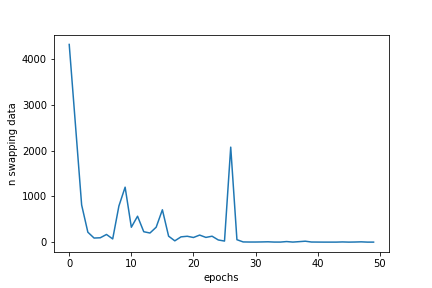
\includegraphics[clip,width=8.5cm]{swapdata.png}
		\caption{データの入れ替え数 (横軸:epoch, 縦軸:データ数)}
		\label{fig:swapdata}
	\end{center}
\end{figure}

図\ref{fig:swapdata}の入れ替えたデータの数では, 初期に4000枚以上の入れ替えが起こっていた. 中期にも2000枚の入れ替えが起こっているが, いづれも図\ref{fig:accuracy}の精度が落ちる時期と重なっている.

\begin{figure}[tb]
	\begin{center}
		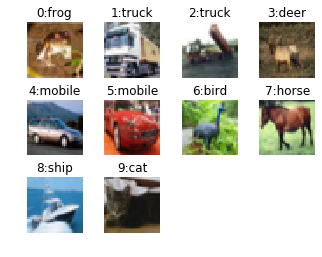
\includegraphics[clip,width=8.5cm]{dataimage.png}
		\caption{データセットAの例, 先頭10件 (index:label)}
		\label{fig:dataimage}
	\end{center}
\end{figure}

\begin{figure}[tb]
	\begin{center}
		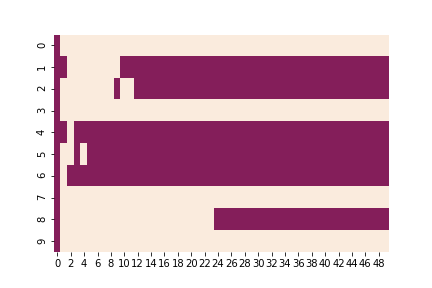
\includegraphics[clip,width=8.5cm]{swap_map.png}
		\caption{データの入れ替え例 (横軸:epoch, 縦軸:index) データセットAの先頭10件のデータの入れ替え履歴. 赤がA, 白がBに属していることを示す}
		\label{fig:swapmap}
	\end{center}
\end{figure}

具体的なデータの入れ替えとして図\ref{fig:dataimage}にデータセットAの画像と図\ref{fig:swapmap}にその入れ替えの過程を示した. 分類を間違えてデータセットBに移動した後, 学習が進んでAに戻っているものもあった. 戻ったデータは, 自動車, トラック, 船などの機械で, この例では動物は学習できていない傾向にあった.

% \section{前回からの進捗}
% あれば報告


\section{考察:現在の問題点}
% 精度が出ない,とかだけではなく自分なりの考察を示す
データの入れ替えを分析すると, 機械クラスが簡単で, 動物クラスが難しいという例が見られた.

しかし入れ替えを行ったときの精度が著しく落ちる原因がまだ分かっていない.
\begin{itemize}
	\item {最適化関数が働いていない}
	\item {表現力が高すぎて過学習している}
\end{itemize}
などが考えられる.

\section{今後の予定}
% なんとなくなんかの勉強をするとかではなく具体的に
\begin{itemize}
	\item {ソースコードに不備がないか確認}
	\item {データの分類難易度の大域的な確認}
\end{itemize}

\section{ソースコード}
% 埋め込みでもGitでもいいので参照できるように

CNNのPytorchでの実装をコード\ref{model_cnn}に示す.

\begin{lstlisting}[caption=cnn,label=model_cnn]
class CNN(nn.Module):
  def __init__(self):
    super(CNN, self).__init__()
    self.model = nn.Sequential(
      nn.Conv2d(3, 64, 3, padding=1),
      nn.ReLU(),
      nn.Conv2d(64, 64, 3, padding=1),
      nn.ReLU(),
      nn.BatchNorm2d(64),
      nn.Conv2d(64, 64, 3, padding=1),
      nn.ReLU(),
      nn.MaxPool2d(2),
      nn.Dropout(0.25),

      nn.Conv2d(64, 128, 3, padding=1),
      nn.ReLU(),
      nn.Conv2d(128, 128, 3, padding=1),
      nn.ReLU(),
      nn.BatchNorm2d(128),
      nn.Conv2d(128, 128, 3, padding=1),
      nn.ReLU(),
      nn.MaxPool2d(2),
      nn.Dropout(0.25),

      nn.Conv2d(128, 256, 3, padding=1),
      nn.ReLU(),
      nn.Conv2d(256, 256, 3, padding=1),
      nn.ReLU(),
      nn.BatchNorm2d(256),
      nn.Conv2d(256, 256, 3, padding=1),
      nn.ReLU(),
      nn.Conv2d(256, 256, 3, padding=1),
      nn.ReLU(),
      nn.Conv2d(256, 256, 3, padding=1),
      nn.ReLU(),
      nn.BatchNorm2d(256),
      nn.Conv2d(256, 512, 3, padding=1),
      nn.ReLU(),
      nn.Conv2d(512, 512, 3, padding=1),
      nn.ReLU(),
      nn.AvgPool2d(8)
    )
    self.pc = nn.Sequential(
      nn.Linear(512, 1024),
      nn.Dropout(0.5),
      nn.Linear(1024, 1024),
      nn.Dropout(0.5),
      nn.Linear(1024, 10),
      nn.Softmax()
    )

  def forward(self, x):
    x = self.model(x)
    x = x.view(-1, 512)
    x = self.pc(x)
    return x
\end{lstlisting}


	% 参考文献リスト
	\bibliographystyle{unsrt}
	\bibliography{ref}
\end{document}
